% Format teze zasnovan je na paketu memoir
% http://tug.ctan.org/macros/latex/contrib/memoir/memman.pdf ili
% http://texdoc.net/texmf-dist/doc/latex/memoir/memman.pdf
% 
% Prilikom zadavanja klase memoir, navedenim opcijama se podešava 
% veličina slova (12pt) i jednostrano štampanje (oneside).
% Ove parametre možete menjati samo ako pravite nezvanične verzije
% mastera za privatnu upotrebu (na primer, u b5 varijanti ima smisla 
% smanjiti 
\documentclass[12pt,oneside]{memoir} 




% Paket koji definiše sve specifičnosti master rada Matematičkog fakulteta
\usepackage[latinica]{matfmaster} 
%
% Podrazumevano pismo je ćirilica.
%   Ako koristite pdflatex, a ne xetex, sav latinički tekst na srpskom jeziku
%   treba biti okružen sa \lat{...} ili \begin{latinica}...\end{latinica}.
%
% Opicija [latinica]:
%   ako želite da pišete latiniciom, dodajte opciju "latinica" tj.
%   prethodni paket uključite pomoću: \usepackage[latinica]{matfmaster}.
%   Ako koristite pdflatex, a ne xetex, sav ćirilički tekst treba biti
%   okružen sa \cir{...} ili \begin{cirilica}...\end{cirilica}.
%
% Opcija [biblatex]:
%   ako želite da koristite reference na više jezika i umesto paketa
%   bibtex da koristite BibLaTeX/Biber, dodajte opciju "biblatex" tj.
%   prethodni paket uključite pomoću: \usepackage[biblatex]{matfmaster}
%
% Opcija [b5paper]:
%   ako želite da napravite verziju teze u manjem (b5) formatu, navedite
%   opciju "b5paper", tj. prethodni paket uključite pomoću: 
%   \usepackage[b5paper]{matfmaster}. Tada ima smisla razmisliti o promeni
%   veličine slova (izmenom opcije 12pt na 11pt u \documentclass{memoir}).
%
% Naravno, opcije je moguće kombinovati.
% Npr. \usepackage[b5paper,biblatex]{matfmaster}







% Datoteka sa literaturom u BibTex tj. BibLaTeX/Biber formatu
\bib{marina-master}

% Ime kandidata na srpskom jeziku (u odabranom pismu)
\autor{Marina R. Nikolić}
% Naslov teze na srpskom jeziku (u odabranom pismu)
\naslov{Prikupljanje i prikaz podataka o izvršavanju programa}
% Godina u kojoj je teza predana komisiji
\godina{2018}
% Ime i afilijacija mentora (u odabranom pismu)
\mentor{dr Milena \textsc{Vujošević Janičić}, docent\\ Univerzitet u Beogradu, Matematički fakultet}
% Ime i afilijacija prvog člana komisije (u odabranom pismu)
\komisijaA{dr Filip \textsc{Marić}, vanredni profesor\\ Univerzitet u Beogradu, Matematički fakultet}
% Ime i afilijacija drugog člana komisije (u odabranom pismu)
\komisijaB{dr Milan \textsc{Banković}, docent\\ Univerzitet u Beogradu, Matematički fakultet}
% Ime i afilijacija trećeg člana komisije (opciono)
% \komisijaC{}
% Ime i afilijacija četvrtog člana komisije (opciono)
% \komisijaD{}
% Datum odbrane (odkomentarisati narednu liniju i upisati datum odbrane ako je poznat)
% \datumodbrane{}

% Apstrakt na srpskom jeziku (u odabranom pismu)
\apstr{tekst apstrakta rada
}

% Ključne reči na srpskom jeziku (u odabranom pismu)
\kljucnereci{profajliranje, pokrivenost koda, GCC, GCOV}

\begin{document}
% ==============================================================================
% Uvodni deo teze
\frontmatter
% ==============================================================================
% Naslovna strana
\naslovna
% Strana sa podacima o mentoru i članovima komisije
\komisija
% Strana sa posvetom (u odabranom pismu)
\posveta{Mentoru za predanost i pomoć, firmi za resurse, porodici i prijateljima za podršku}
% Strana sa podacima o disertaciji na srpskom jeziku
\apstrakt
% Sadržaj teze
\tableofcontents

% ==============================================================================
% Glavni deo teze
\mainmatter
% ==============================================================================

% ------------------------------------------------------------------------------
\chapter{Uvod}
% ------------------------------------------------------------------------------


\begin{enumerate}
\item kratak opis o čemu će biti reči u daljem tekstu
\item iako vidim da je popularno po master radovim ada se piše po poglavljima ovde (tipa, u poglavlju X je opisano to i to), ja bih uvod radije sročila kao pričicu koja prati rad
\item ovde bih dodala na samom početku i na samom kraju značaj teme kao takve i naravno značaj mog doprinosa ( na kraju zbog efekta)
\end{enumerate}


% ------------------------------------------------------------------------------
\chapter{Profajliranje, pokrivenost koda i kako sad radi GCC}
\label{chp:profajliranje}
% ------------------------------------------------------------------------------

\section{Profajliranje i pokrivenost koda}


Na jednom predavanju na Matematičkom fakultetu, davne 2017 godine, jedan profesor po imenu Saša Malkov je rekao svojim studenatima: "Razvoj softvera nije samo sedenje i kuckanje po tastaturi. Videćete jednog dana kad počnete da radite nešto ozbiljno.".
Tema ovog rada i projekat na kome je utemeljen su ponikli iz te rečenice, ali već je sam proces izrade projekta prvi nepobitno dokazao to tvrđenje. U vrlo ranoj fazi razvoja, već su se mogle nazreti razne faze kroz koje je ovaj projekat, kao i naravno svi ostali, morao proći, kao i to da je raspodela kako obima, tako i važnosti segmenata razvoja softvera, dosta drugačija od ustaljenog mišljenja među laicima, pre svega klijentima.


Za proizvodnju kvalitetnog i dugotrajnog softvera, jako važni segmenti razvoja su: planiranje, analiza i usklađivanje sa zahtevima klijenata, testiranje, analiza performasi, optimizacija, održavanje, … Kompleksnost ovih segmenta, kao i važnost njihovog olakšavanja, najbolje mogu uvideti i razumeti ljudi koji se bave razvojem softvera. Težnja svakog čoveka je je da olakša sebi posao. Bilo da govorimo o jednostavnom programeru koji piše sebi sitne skripte koje će umesto njega odrađivati jednostavne a repetativne zadatke, ili pak o onim ambicioznijim, koji žele da naprave velike promene za celu računarsku zajednicu. Zbog toga i sami razvijaoci softvera posvećuju svoje vreme i trud osmišljavanju novih načina da olakšaju svojim kolegama i sebi sve gore navedene segmente razvoja softvera. Potpuno je prirodno i logično da je za procese konstrukcije planova i analiza potrebno dosta vremena, razmišljanja i takozvanih "menadžerskih gena". Malo je teže pretpostaviti da je jednako zahtevno sprovesti procese testiranja i optimizacije. Još pre nego što samo pisanje i započne, važno je dobro proceniti koje segmente koda i kojom metodom testirati/optimizovati, a da bi se to učinilo, mora se dati odgovor na mnoga pitanja poput: "Kako pokriti najosetljivija mesta unit testovima?" ili "Koje rutine je najvažnije optimizovati?". To naravno nije lako. Neophodno je znati najsitnije detalje o originalnom softveru, a to je, mora se priznati, osetljiva tačka i samom razvojnom timu. Dobar odabir je, dakle, nepobitno uslovljen dobrim poznavanjem samog softvera, njegovih osobina i ponašanja. Ovim, naizgled nerešivim problemom, uspešno se bavi analiza programa.


Analiza programa predstavlja automatizovani proces analiziranja raznih aspekata softvera, pre svega njegovog ponašanja, u različitim slučajevima upotrebe, u cilju pružanja pomoći programerima pri testiranju korektnosti, naročito eksterno nabavljenih delova softvera, proceni performansi i optimizaciji. Pruža korisne informacije o raspodeli potrošnje resursa, čvorovima ekstremne potrošnje, potencijalnim kritičnim segmentima izvršavanja, korektnosti toka izvršavanja i slično. Pomalo nalik na projekat veštačke intaligencije, njen put vodi ka stvaranju pametnog kompajlera, koji bi mogao automatski generisati vrlo efikasan, a pouzdan kod. Njene mogućnosti su i u ovom trenutku dosta velike, ali ako se uzme u obzir da je ovo disciplina u razvoju, neosporno se može tvrditi da je njena budućnost revolucionarna. Analiza programa je veoma širok pojam, koji obuhvata pregršt vrlo raznovrsnih metoda, ali se takođe može veoma precizno podeliti na dva osnovna tipa. To su statička i dinamička analiza.


Statička analiza programa obuhvata sve metode i tehnike utvrđivanja ponašanja programa, za koje ga nije potrebno izvršiti. Sve procedure se vrše nad izvornim kodom i, vešto prikupljajući podatke o njegovoj strukturi, generišu korisne informacije o mogućim ishodima njegovog budućeg izvršavanja. Primer su mnogobrojne softverske metrike koje na osnovu podataka o broju linija, klasa ili metoda, izračunavaju "statistički kvalitet" softvera. Njena glavna prednost počiva baš na tome, što kod nije potrebno izvršiti. Na prvi pogled deluje kao da je teško pronaći primer kada je ovakvo ograničenje nametnuto, ali pri razvoju velikih i skupih softvera neretko se dešava da pojedini delovi razvoja bivaju uskraćeni za "probu", naročito u realnim okruženjima. Dovoljno je zamisliti razvoj softera za automatsko navođenje rakete. Vrlo realan zadatak je napisati manji program za izračunavanje potrošnje goriva prilikom neke vožnje. Testiranje ovakvog jednog programa se naravno vrši u najvećoj meri na simulatorima. Vrlo je zdravorazumski pretpostaviti da se nakon svake iteracije pisanja koda neće pokretati prava raketa za potrebe testiranja, a takođe je vrlo zdravorazumski pretpostaviti da simulator ne pruža potpuno jednako okruženje, niti obuhvata sve alternativne slučajeve upotrebe jedene rakete. Sa druge strane, ukoliko uzmemo u obzir činjenicu da vreme izvršavanja proizvoljnog programa može biti proizvoljno dugo, iz neneophodnosti izvršavanja, lako možemo izvesti još jednu veliku prednost statičke analize, a to je brzina. U savremenom svetu, važi pravilo: ,,Vreme je novac, a novac pokreće svet.”. Iz nenophpodnosti izvršavanja, proističe još jedna velika prednost statičke analize, koja je samo naizgled manje važna od prethodne, a to je nepristrasnost. Nezavisnost od ulaznih podataka i okruženja, čini je savršenim oružjem za borbu protiv graničnih slučajeva ("edge/corner cases"). Naravno, ovaj brzi ekonomični nepristrasni pristup dolazi sa određenom cenom, koja se ponekad plati kasnije, a tada je mnogo skuplje. Njena uska veza sa statistikom kao naukom, koja vodi u nepreciznost, kao i manjak informativnosti o "realnim slučajevima upotrebe" može biti pogubna neiskusnim razvojnim timovima. Stoga se ne sme zaboraviti da se statička analiza zaustavlja na predviđanju. Njeni rezultati su teorijski, ne eksperimentalni, i uvek se trebaju uzimati sa određenom dozom skeptičnosti.


Dinamička analiza \cite{Gupta} programa obuhvata sve metode i tehnike prikupljanja podataka o programu tokom njegovog izvršavanja i utvrđivanja ponašanja programa na osnovu tih podataka. Procedure uglavnom započinju u fazi prevođenja, ali najvažniji deo se obavlja u toku i nakon izvršavanja. Pored strukture koda i statičkih podataka, na njen ishod utiču i ulazne vrednosti, kao i parametri okruženja. Testovi jedinica koda, sistemski testovi i testovi prihvatljivosti koriste isključivo ovaj vid analize programa. Sve njene glavne prednosti u odnosu na statičku analizu, proističu iz uticaja "realnih parametara". Određene mane softverskih rešenja ispoljavaju se samo u toku rada tog softvera, a mnoge i proističu baš iz spoljnih faktora ili veze sa njima. Iskreni odgovor jednog ozbiljnog proizvođača ili razvijaoca softvera će veoma često biti da je najveći neuspeh višegodišnji rad na statistički savršenom softveru, kome je jedina mana neprimenljivost u praksi. Troši se mnogo novca na marketinška istraživanja, analize zahteva korisnika ili naručioca, ili iscrpne popise slučajeva upotrebe, ali to neretko nije dovoljno. Pojedini faktori okruženja, kao što je na primer realnost jedne jedinice iz skupa obrade, takozvane "lažne negativne vrednosti" (false negative), jednostavno se previše dobro sakriju u moru statističkih podataka. To vodi u beskrajni začarani krug prilagođavanja i održavanja gotovog proizvoda, koji se veoma često završi odustajanjem kada se novac potroši ili se pronađe nešto bolje. Stoga, testiranja u realnom okruženju su veoma važna, a kako su po svojoj prirodi ograničena resursima, važno je iz njih ekstrahovati što više informacija za naredne iteracije razvoja. Za taj sitni detalj, dinamička analiza programa je neizostavni i nezamenljivi faktor. Još jedna važna prednost koja se na prvi pogled ne vidi tako jasno, jeste to da se dinamička analiza vrši nad izvršnim programom, a ne izvornim kodom. To je čini univerzalnijom, jer se može primenjivati i na programe sa "zatvorenim" kodom. U praksi, pisanje svake linije koda nekog softvera je luksuz koji troši previše vremena i novca. U današnje vreme, kada je parola: "Pisati kod brzo i jeftino inače će konkurencija to učiniti" toliko zaživela, takozvano "recikliranje koda" je postalo jedini dovoljno kompetetivni način proizvodnje. Ovaj princip nije karakteristika samo softverske industrije, a za ilustraciju se može iskoristiti čak i gradski prevoz. Dovoljno je uporediti cenu jedne karte za autobus sa cenom goriva i održavanja automobila, na relaciji od svega par kilometara. Korišćenje javnog prevoza je jeftinije jer se trošak prevoza deli na više osoba. Tako je putnicima povoljnije, a isplati se veoma i prevozniku, jer svoj proizvod ne ustupa za tačan iznos pojedinačnog dela. U ilustraciju je namerno ubačena i cena održavanja, jer je i u softverskoj industriji to najskuplji faktor. Može se dakle zaključiti, da se u svom rešenju, razvojni timovi moraju poprilično osloniti i na eksteno nabavljene komponente, kod kojih se može dobiti samo izvršna verzija. Izvorni kod je strogo čuvana tajna proizvođača. Procene kvaliteta pre integracije, kao i testiranje kompatibilnosti sa ostatkom softvera, jesino se mogu obaviti dinamičkim pristupom. Time ona zasluženo odnosi pobedu u katgoriji univerzalnosti. Najveća mana ovog pristupa jeste potencijalni osećaj lažne sigurnosti. Nažalost, to je neizostavna stavka svakog testiranja. Neiskusni razvojni timovi se mogu previse osloniti na rezultate analize i time prevideti činjenicu da je ona ipak automatizovani proces i samim tim ne može garantovati stoprocentnu tačnost. Alati koji je vrše su takođe proizvod nekog razvojnog tima, i samim tim jednako podložni greškama koliko i kod koji se njima analizira. Posebno mesto u tehnikama dinamičke analize ima profajliranje, i njimu će ovaj rad biti u potpunosti posvećen. 


Profajliranje\cite{PGO}\cite{Verifikacija} predstavlja prikupljanje raznovrsnih podataka iz izvršavanja programa u realnom ili simuliranom okruženju, koji pružaju uvid u tok i performanse rada programa. Obradom ovih podataka, dobiaju se vredne informacije o vremenskim i memorijskim zahtevima programa, složenosti i iskorišćenosti pojedinih delova koda i slično. Rezulatati radi alata za profajliranje predstavljaju neizostavnu i nezamenljivu vodilju za procese testiranja i optimizacije, pre svega jer jasno pokazuju kojim delovima koda su ti procesi najpotrebniji. Ulazne vrednosti i parametri okruženja, zajedno sa kodom programa, jedinstveno određuju tok izvršavanja. Uočavanje pozitivnih podataka o izvršavanju mimo predviđenog toka, ili negativnih u njegovoj unutrašnjosti, za unapred određen slučaj upotrebe, je stoga dobar pokazatelj da se u kodu nalaze greške. Štaviše, pruža i dodatnu olakšicu za budući proces debagovanja, sužavanjem oblasti pretrage. Detekcija memorijski ili vremenski izrazito zahtevnijih segmenata, kao i segmenata koji se veoma često izvršavaju usmerava pažnju razvojnog tima na neophodnost optimizacije, pritom takođe obezbeđujući dodatnu informaciju gde je ona i koliko potrebna. Poređenjem performasi različitih verzija koda, može se izvršiti dobra procena kvaliteta i odabir odgovarajućeg algoritma u ranim fazama, kada je njegova zamena još uvek dovoljno jeftina. Smernice koje profajleri daju mogu znatno "očistiti" kod od nepotrebnih grananja, invarijanti petlji pogrešno smeštenih unutar same petlje, "mrtvog koda" i mnogih drugih sitnih propusta. Stoga značajno olakšavaju i proces refaktorisanja koda, koji je često veoma dug i mukotrpan posao. Vrši se alatom koji se naziva profajler i sastoji se od tri usko spregnute faze: instrumentalizacija, prikupljanje i obrada podataka. 


Instrumentalizacija\cite{SCI} koda predstavlja sposobnost merenja karakteristika programa, koja se postiže ubacivanjem dodatnih instrukcija u program tokom prevođenja. Instrukcije predstavlju kod inicijalizacija određenih dodatnih struktura za instrumentalizaciju i pravila za njihovo popunjavanje. Dodatne strukture služe kao skladišta za metapodatke, a uputstvo za korišćenje nagoveštava programu kako da ih popuni, jer je taj posao poveren isključivo njemu. Možda na prvi pogled deluje kao neoptimalno opterećivanje programa, ali postoji mnogo faktora koji to neosporno opovrgavaju. Pre svega, tu je faktor bezbednosti. Neograničen pristup internim podacima jednog programa ne sme imati niko sem njega samog. To bi stvorilo veoma  plodno tle za razvoj malicioznog softvera koji bi zloupotrebio ovaj bezbednosni propust, bilo napadajući alat za instrumentalizaciju, bilo poruke koje razmenjuje sa instrumentalizovanim programom. Zaštita u vidu šifrovanja bi zahtevala dodatno trošenje resursa, što nije isplativo. Pored bezbednosnog aspekta, bitan faktor je i sinhronizacija. U sistemu sa eksternim alatom, usklađivanje čitanja i pisanja memorijskih segmenata dodeljenih programu bi iziskivala dodatno trošenje procesorskog vremena i memorije, a i zaključavanje bi povećalo vremensku složenost. 


Faza prikupljanja podataka obuhvata: čitanje dodatnih struktura sa metapodacima, njihovo konvertovanje u pogodniji oblik i eksterno skladištenje. Da bi oblik bio pogodan, neophodno je da predstavlja savršeni balans između veličine, koja treba biti što manja, i informativnosti, koja treba biti što veća. Ukoliko neki podaci mogu da se izvedu iz ostalih, oni se eliminišu. Lokacija podataka u eksternom skladištu predstavlja memorijski besplatan podatak, koji omogućava dodatnu kompresiju bez gubitka na informativnosti. Ova faza je takođe poverena samom programu, iz istih razloga kao i instrumentalizacija. 


Produkt prve dve faze su sirovi podaci, koji u sebi nose informacije o karakteristikama programa u realnim slučajevima upotrebe, ali kako se podaci prikupljaju samo ako program ima još jednu dodatnu funkciju, tj. usput mora i da prikuplja svoje metapodatke, ukupna slika se može malo iskriviti u procesu. Uticaj se, nažalost, ne može u potpunosti ukloniti, ali se mora svesti na granicu prihvatljivosti. Ispravna instrumentalizacija ne sme nikako uticati na funkcionalnost programa, a usporavanje mora biti dovoljno malo da ne utiče na rad programa. 


Poslednja faza predstavlja obradu sirovih podataka do korisne informacije. Krajnji proizvod predstavlja jedan ili više izveštaja u formatu pogodnom prvenstveno za razvojni tim, ne za računar. Osnovne karakteristike izveštaja treba da budu: uniformnost, preglednost, povišena (vraćanje izvedenih podataka) ili snižena informativnost (filtriranje podataka po kategorijama), unija pojedinačnih i statističkih prikaza i slično. Ovu fazu obično obavljaju eksterni alati, jer je potpuno nezavisna od izvršavanja programa i njegove interne memorije. U zavisnosti od toga koje se karakteristike mere i potreba korisnika, krajnji izveštaji variraju od jednorečeničnih ispisa, preko čitavih zbirki fajlova, do interaktivnih aplikacija. Mogu se meriti razne karakteristike, poput na primer memorijskih zahteva ili tragova izvršavanja, ali se po informativnosti i univerzalnosti primene naročiito ističe pokrivenost koda.


Pokrivenost koda \cite{Introduction} \cite{Testing} \cite{Ecl} \cite{Warrning} \cite{Misuse} \cite{Pizza} predstavlja "stepen izvršenosti koda". Izračunava se kao odnos broja izvršenih i neizvršenih linija, blokova, grana ili funkcija i izražava se u procentima. U strogom smislu, pokrivenost koda je jedan jedini broj, dobijen merenjem nad celim sistemom. Taj broj je sam po sebi veoma informativan. Što je pokrivenost manja, to je verovatnoća da u kodu postoje ozbiljne greške u logici veća. 


Međutim, nakon merenja na celom skupu, poželjno je uraditi i merenja na manjim segmentima: komponentama, klasama, funkcijama, ... Time se mogu uočiti propusti koje ukupna statistika sakrije. Na primer, ukoliko je stil pisanja koda takav da se po fajlovima grupišu slični metodi iz različitih klasa, ovakvim pristupom mogu se bolje detektovati slabo ili nimalo korišćene klase, ili objekti koji se prave i uništavaju bez da utiču na ukupnu funkcionalnost. Takođe, čisti podaci o konkretnim linijama koje su i koliko puta izvršavale, takođe može otkriti neki satistički zakopan detalj. Pronalazak invarijanti petlje slučajno smeštenih u njenu unutrašnjost ili bespotrebnih grananja koja se svedu na isti krajnji rezultat, samo su neki od primera. Stoga, pokrivenost koda ne treba shvatati samo u svom najužem smislu, već maksimalno iskoristiti bogati rudnik nformacija koji predstavlja. Uzroci neočikivane pokrivenosti mogu biti veoma raznovrsni. U daljem tekstu biće predstavljeno nekoliko primera. 


Stariji softveri koji se duže vreme održavaju, neretko sadrže visok procenat takozvanih "tragova iz prošlosti". Smenom razvojnih timova, naročito u okruženjima koja ne podržavaju detaljno dokumentovanje učinka, često se gube informacije o funkcionalnosti pojedinih delova koda. Usled nedostatka informacija, većina "naslednika", uglavnom nema hrabrosti da eliminiše ili zamenjuje delove koda, već se uglavnom vrši dodavanje. Funkcije ili klase, a neretko i čitave komponente, tako postaju mrtav kod, sa jedinom ulogom otežavanja održavanja ili debagovanja. Ovakvi softveri imaju naročito malu pokrivenost. 


Da se preterani perfekcionizam plaća slabim performansama, opšte je poznat zakon u razvojnim kugovima. Iskustvom se stiče osećaj za balans između preciznosti i brzine, ali nikada savršen. Ukoliko se uzme u obzir još i težina problema određivanja svih mogućih, ali realnih, slučajeva upotrebe, postaje prilično jasno koliko je velika verovatnoća da u tom procesu razvojni tim ostane "izgubljen u grananju".  Iako naizgled mali problem, suvišna grananja mogu proizvesti ogromne količine mrtvog koda, od linija pa do čitavih klasa ili komponenti pisanih isključivo za te specijalne slučajeve. To znatno otežava održavanje koda, debagovanje i refaktorisanje. Mala pokrivenost može biti koristan simptom, a podaci izvršanja linija locirati mesto na kome treba delovati. 


Današnji sistemi se ne mogu zamisliti bez konkurentnog i paralelnog izvršavanja. Porast efikasnosti koji se njima postižu je toliko značajan da baca senku na sve nove potencijalne probleme koje je donelo sa sobom. Živa i mrtva zaključavanja, kao i takozvana trka za resurse, samo su neki od njih. Potencijal ovih problema je toliko moćan, da mogu blokirati čitav sistem, a rano otkrivanje, pre nastanka, je praktično nemoguće. Procesor je jedini koji odlučuje koji će se proces, kada i koliko izvršavati, a na programeru je da se zaštiti sitnim trikovima poput obezbeđivanja atomičnosti ili prioriteta onoliko koliko može. Međutim, i pored maksimalnog truda njihovih autora, ponekad se jednostavno proces ne uspe izboriti za svoje vreme na procesoru. Takvi kodovi imaju izuzetno niske pokrivenosti, a najbolji pokazatelj su pokrivenosti pojedinačnih izvršavanja koje iznose nula procenata. Prilikom rada sa nitima, niske pokrivenosti mogu biti simptom i preopterećenosti. 


Najozbiljniji problemi koji uzrokuju malu pokrivenost su ipak takozvane "greške u logici". One mogu varirati, od pogrešno definisanih uslova u granama ili petljama do potpuno promašenih algoritama. Neočekivana generalna pokrivenost može biti dobar signal da u kodu ima ovakvih grešaka. Pokrivenost manja od očekivane može na primer insinuirati poziv pogrešnih funkcija, ulazak u neproduktivnu granu ili prevremeni izlazak iz programa. Veća pokrivenost od očekivane može biti simptom nepravilnog rada uslova u naredbi grananja, loše konstruisanih provera u kodu i još mnogo toga. Kako uzroci mogu biti veoma raznovrsni, dobro je pored generalne, meriti i pokrivenosti na segmentima. Kombinovanjem svih rezultata, sužava se oblast pretrage i lako locira greška u logici. 


Jedini svedok o kvalitetu koda pre nego što ode u produkciju je dobar test. Međutim podaci dobijeni testiranjem ne svedoče samo o kvalitetu softvera, već i o kvalitetu samih testova. Testovi se često sami ne testiraju dovoljno dobro, a posledice mogu biti veoma ozbiljne. Lažan negativan rezultat može uzrokovati veliku bespotrebnu potrošnju vremena i novca na traženje nepostojeće greške u kodu. Lažan pozitivan rezultat može imati još i ozbiljnije posledice, čija težina zavisi od važnosti samog softvera. Stoga je veoma korisno primeniti tehniku određivanja pokrivenosti koda i na testove, a ne samo na softver. Mala pokrivenost je dobar indikator da u kodu postoje segmenti koji nisu testirani, koji su samim tim potencijalna opasnost.

 
Računanjem pojedinačnih pokrivenosti možemo doći i do informacija o često korišćenim segmentima koda. One umnogome olakšavaju razvojnom timu prilikom donošenja odluka vezanih za vremensku optimizaciju. Kombinovanjem sa podacima za pojedinačne linije koje recimo alociraju memoriju, mogu se pronaći memoriski zahtevni segmenti koji su idealni kandidati za prostornu optimizaciju. 


Najsitniji podaci, poput podataka o izvršavanju pojedinih linija ili blokova se mogu veoma dobro koristiti za refaktorisanje. Odstranjivanje mrtvog koda ili razbijanje preopterećene funkcije, samo su neke od sitnica koje za održavanje život znače, a uz pokrivenost koda su prilično olakšane. 


Raznovrsnost gore navedenih primera nepobitno dokazuje veliki značaj i potencijal pokrivenosti koda. Stoga će, poptuno opravdano, na nju biti u poptunosti skoncentrisan ostatak ovog rada. 


Poznatiji prevodioci, poput GCCa, ICCa i Clanga uglavnom u određenoj meri poseduju ugrađenu podršku za testiranje pokrivenosti koda. Projekat LLVM trenutno ima najraznovrsniju ponudu, koja obuhvata i statički i dinamički pristup, uključujući i testiranje u toku izvršavanja. Sa druge strane, GCC trenutno podržava samo statičko testiranje pokrivenosti nakon izvršavanja programa, ali ga odlikuju znatno bolje performance, pre svega u pogledu memorijske zahtevnosti. Prkupljanje i obrada podataka o pokrivenosti koda u toku izvršavanja programa korišćenjem tehnika GCCa, kombinuje dobru ideju projekta LLVM i dobre tehnike prevodioca GCC, čime prednjači i u oblasti mogućnosti i u oblasti performansi. U okviru projekta na kome je utemeljen ovaj rad, izvršena je detaljna analiza postojećih mogućnosti u okviru prevodioca GCC i implementirana je podrška za prikupljanje podataka u toku izvršavanja, kao i novi, unapređeni alat za njihov vizuelni prikaz.


\section{Postojeća rešenja u okviru GCCa}


Programski prevodilac GCC sadrži ugrađenu podršku za testiranje pokrivenosti koda, integrisanu u statičku biblioteku za prikupljanje podataka po imenu libgcov i alat za vizuelni prikaz podataka GCOV \cite{GCOV} \cite{CodeCoverage}.


Metapodaci izvršavanja programa čuvaju se u deljenoj memoriju programa, u listi posebnih, globalno definisanih struktura tipa gcov\_info, čija se inicijalizacija ugrađuje u binarni kod prevođenjem sa posebnim flegovima za instrumentalizaciju: -fprofile-arcs -ftest-coverage. Flegovi se navode tokom prevođenja izvornog koda do objektnog fajla, a simboli koji se njima unose razrešavanju se kasnije u fazi linkovanja. 


Pored ubrizgavanja instrukcija u binarni kod programa, flegovi za instrumentalizaciju imaju još jedan važan zadatak, a to je kreiranje jednog dodatnog fajla, odmah pored njemu odgovarajućeg fajla izvornog koda, sa ekstenzijom gcno. To je relativno mali, binarni fajl, koji sadrži sve neophodne statičke informacije o strukturi izvornog koda čijim prevođenjem nastaje. Njegova glavna uloga jeste da predstavlja kalup u koji će se na unapred previđenim mestima kasnije "izlivati" podaci dobijeni dinamički u toku izvršavanja. Format gcno fajla je utvrđen zajedničkim standardom gcc-a i alata gcov, koji je specijalizovan i za njegovo tumačenje. Veoma je nečitljiv ljudskom oku, što je uzrokovano maksimalnim stepenom kompresije podataka. Korišćenje specijalnih oznaka, korišćenje pozicije kao interpretacije podatka, kao i pažljivo odabrani minimalni skup potrebnih informacija o strukturi, samo su neki od tehnika kompresije korišćenih u cilju maksimalne štednje memorije. Posebno je važno napomenuti, da je čuvanje podataka o strukturi u vidu eksternih binarnih fajlova osnovni uzrok velike memorisjke pobede gcc instrumentalizacije nad clang-ovim profajliranjem, pomenute na kraju prethodnog poglavlja, jer garantuje bezbednost od eksplozije veličine samog programa. Dovoljno uvećanje izvršnog fajla može dosvesti do nepravilnosti u radu, a kako memoriski zahtevniji instrumnatlizovani program se ponaša drukčije od regilarnog, rezultati testiranja mogu prikazivati blago iskrivljenu sliku, što nije ispravno. Naročito, na sistemima sa veoma ograničenim memorijskim prostorom, gcc instrumentalizacija je jedina moguća. 


Svaka struktura tipa gcov\_info iz liste, odgovara tačnom jednom instrumentalizovanom objetnom fajlu koji učestvuje u izgradnji programa. Pored osnovnih podataka poput imena fajla ili verzije alata, svaka struktura tipa gcov\_info sadrži i pokazivač na niz struktura tipa gcov\_fn\_info, u kojima se skladišti po nekoliko posebnih brojača za svaku funkciju tog fajla. Na osnovu vrednosti u njima, može se konstruisati podatak o količini izvršavanja bilo koje jedinice koda u okviru te funkcije. Tokom rada programa, vredosti u brojačima se konstantno ažuriraju, i u svakom trenutku odražavaju realno stanje izvršavanja. Ti podaci predstavljaju jezgro informacije o pokrivenosti koda, ali njih eksterni alat poput GCOVa ne može direktno koristiti iz više razloga. Prvi razlog je bezbednosne prirode, i velikom merom je obrazložen u prethodnom poglavlju. Eksternim alatima se ni u kom slučaju ne treba obezbediti čitanje internih podataka programa. Detaljno je obrazloženo i pitanje sinhronizacije pisanja i čitanja, koje važi i u ovom slučaju. Naposletku, ovim pristupom bi podaci imali poreklo samo iz jednog izvršavanja, a nema razloga ograničavati se na tako nešto. 


Rešenje koje je trenutno implementirano u GCC, upravo iz tih razloga, sadrži jednog "posrednika" između instrumentalizovanog programa i eksternih alata, a to je libgcov. Biblioteka, po svojoj prirodi, se ugrađuje (linkuje) u program i time postaje deo njega, što joj daje ekskluzivno pravo pristupa svim tajnovitim mestima u njegovoj deljenoj memoriji. Njen osnovni zadatak je ekstrakcija podataka iz strukture gcov\_info i njihovo konvertovanje u oblik pogodan za obradu eksternim alatom. Statička funkcija gcov\_at\_exit preuzima vrednosti brojača, računa sumarne i statističke podatke i sve zajedno upisuje u posebni binarni fajl sa ekstenzijom gcda u unapred utvrđenom formatu i na unapred utvrđenoj lokaciji. Format gcda fajla je takođe veoma nečitljiv, usled primene sličnih trikova za kompresiju, kao u slučaju gcno fajla. Generiše se uvek pored objetktong fajla kome odgovara, u slučaju da fajl sa istim imenom i ekstenzijom već ne postoji na toj lokaciji. U slučaju višestrukog pokretanja programa, vrednosti iz predhodnih izvršavanja već se nalaze u gcda fajlu, te se on samo ažurira, a za sumiranje starih i novih podataka, zadužena je druga funkcija po imenu \_\_gcov\_merge\_add\_. Stoga, ukoliko želimo da zanemarimo stare podatke, moramo premestiti ili ukloniti prethodni gcda fajl pre novog pokretanja. 


Na kraju izvršavanja instrumentalizovanog programa, svi podaci potrebni za informisanje razvojnog tima o pokrivenosti njihovog koda, nalaze se na fajl sistemu i mogu se pakovati, premeštati, skladištiti, … To je veoma korisna činjenica, jer otvara nebrojano mnogo mogućnosti kombinovanja rezultata različitih testiranja. Ukoliko postoji potreba da se neki test prekine na određeno vreme i započne novi, gcda fajlovi prvog testa se mogu spakovati na drugu lokaciju, čime će se za drugi test generisati novi, i ponovo prebaciti pored objektnih pred nastavak prvog testa. Za ekonimično skladištenje mogu se koristiti i kompresovane arhive ili eksterni memorijski mediji. Međutim, njihova osnovna funkcija je da predstavljaju materijal koji alat GCOV pretvara u tekstualni izveštaj, pogodniji za ljudsko oko. 


Recept za izveštaj alata GCOV ima svega tri sastojka po izveštaju: jedan izvorni fajl, jedan odgovarajući strukturni fajl (GCov NOtes file - gcno) i jedan fajl sa vrednostima brojača (GCov DAta file - gcda). Poseban tekstualni fajl sa ekstenzijom gcov se kreira za svaki instrumentalizovani fajl izvornog koda. Izveštaj liči veoma na sam izvorni kod, uz dodatak jedne vrednosti ispred svake izvršne linije, koja predstavlja broj puta koliko se ta linija izvršavala. Ukoliko se linija nije izvršila nijednom, ispred nje se se stavlja posebna oznaka sastavljana od pet simbola tarabice. Prvih nekoliko linija izveštaja rezervisano je za stističke podatke o imenima fajlova od kojih je kreiran, dok se na standarni izlaz štampa najvašnija vrednost: odnos broja izvršenih linija i ukupnog broja linija, tj. pokrivenost koda. Na slici \ref{fig:report}, prikazan je primer osnovnog GCOV izveštaja, koji se generiše pozivom alata bez dodatnih opcija. Korišćenjem flegova u pozivu alata, izveštaj se može unaprediti i podacima o blokovima, granama, funcijama i slično.


\begin{figure}[!ht]
  \centering
  \label{fig:report}
  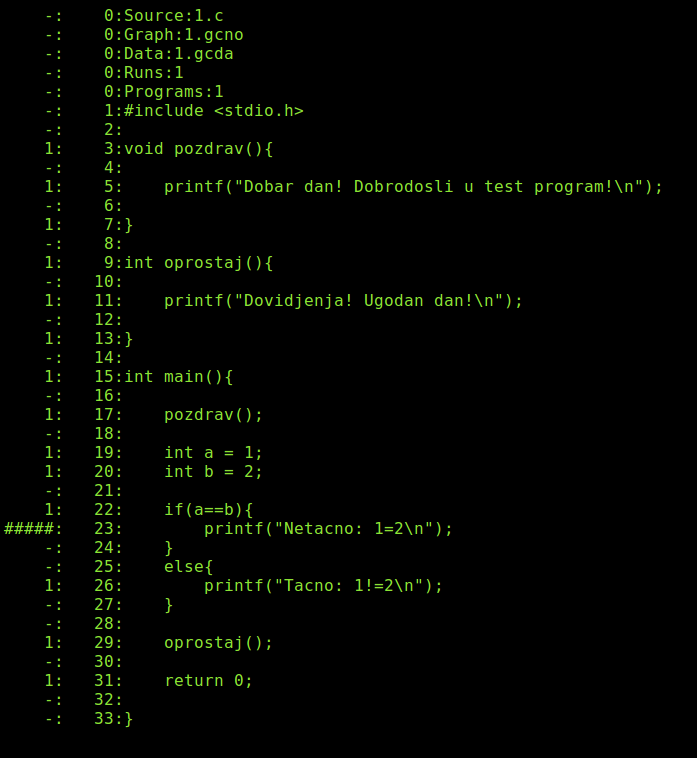
\includegraphics[width=0.5\textwidth]{report.png}
  \caption{report}
\end{figure}


Čitanje podataka iz deljene memorije programa i njihovo skladištenje u gcda fajlove, odvija se na kraju izvršavanja, kao poslednja instrukcija programa pre kraja izvršavanja (at\_exit). Usled toga, iako analiza GCOV alatom nije striktno vezana za vremenski tok izvršavanja, ne može se vršiti pre kraja programa. Ovo je veliki nedostatak, koji u nekim specifičnim slučajevima može poptuno omemogućiti testiranje pokrivenosti koda. Programi kod kojih je na primer vreme rada izuzetno dugo ili su podaci dostupni i/ili korisni samo tokom rada, kao na primer sistemi za rad u realnom vremenu, serveri ili operativni sistemi, ne mogu koristiti statičku instrumentalizaciju na kraju izvršavanja. Ukoliko imaju ograničene memorijske mogućnosti, što je često slučaj na ovakvim sistemima, ne mogu koristiti ni dinamički pristup programskog prevodioca projekta LLVM. Postojanje ovakvih programa, svedoči o važnosti i neophodnosti proširenja mogućnosti instrumentalizacije gcc-a na prikupljanje podataka u toku izvršavanja. 


Sa druge strane, prikaz u vidu pojedinačnih izveštaja za svaki fajl izvornog koda, ima svoje mane. Pojedinačni izveštaji se često nalaze proizvoljno raspršeni po direktorijumu projekta, te je njihov pregled prilično otežan. Dodatne informacije o pokrivenosti pojedinačnih funkcija, koje se dobijaju dodavanjem posebnog flega u poziv alata, kao i ukupna pokrivenost fajla, ne ostaju u izveštajima, već se gube među brojnim drugim ispisima po standardnom izlazu. Povr svega, ukupna statistika se ne računa, te krajnji rezultat ne sadrži istinsku vrednost pokrivenosti koda projekta. Ideja o novom alatu za prikaz GCOV statistike, ponikla je upravo iz potreba da se ove sitne mane prevaziđu. 





% ------------------------------------------------------------------------------
\chapter{Zacetak ideje i trnoviti putevi}
\label{chp:ideja}
% ------------------------------------------------------------------------------

\section{Ideja – dinamicki pristup}

\begin{enumerate}
\item Uvod u moj projekat
\item Šta je ovde drukčije i bolje
\item Samo teorija, bez detalja kako tačno radi šta
\end{enumerate}

\section{Razmatrana rešenja}

\begin{enumerate}
\item Dva puta koja su se predamnom bejaše otvorila – da li napadati GCOV alat ili menjati biblioteku
\item Kako i zašto sam odabrala ovo što sam odabrala
\item Lepa pričica da se pokaže da se ipak ulagalo malo mozga u projekat
\end{enumerate}


% ------------------------------------------------------------------------------
\chapter{Implementacija i analiza}
\label{chp:sprovodenje}
% ------------------------------------------------------------------------------

\section{Implementacija}

\begin{enumerate}
\item Biblioteka
\item GUI (signali za prikupljanje podataka, generisanje izvestaja)
\end{enumerate}

\section{Demonstracija i uputstvo za upotrebu}

\begin{enumerate}
\item primer rada biblioteke I GUI-ja sa slikama
\item dobar moment da se naglasi da rad ima primenu na bilo koji kod
\item ne znam jel smem pominjati digitalnu i ko ga sad koristi
\end{enumerate}

\section{Performanse}

\begin{enumerate}
\item da li smo postigli cilj
\item da li možemo isto što i pre, pa i više
\item memorija I bezbednost – test sa Valgrindom
\item složenost – vremenska i prostorna
\item jednostavnost upoterebe
\item ne bi bilo loše ovde pomenuti LLVM i njihovu runtime instrumentalizaciju 
%(LLVM jede memoriju ko lud, jer podatke dampuje u fajlove ali i ugrađuje u samu binariju koja zato naraste mnogo i pravi probleme, dok GCC sve dampuje u fajlove pa je binarija mala).
\end{enumerate}

\section{Primena}

\begin{enumerate}
\item Gde bi sve ovo moglo da radi
\item Ne znam koliko smem odavati na čemu je testirano I na čemu radi
\item Ideja: Ako bi se ovakav jedan alat unapredio I ugradio npr u pejsmejker da signalizira da nešto ne radi kako treba, to što je runtime prikupljanje moglo bi nekome spasiti život
\end{enumerate}


% ------------------------------------------------------------------------------
\chapter{Zaključak}
% ------------------------------------------------------------------------------


\begin{enumerate}
\item Šta je urađeno
\item Koji je značaj toga što je urađeno (gde sad radi – onliko koliko smem da kazem)
\item Šta bi još moglo da se uradi:
\begin{enumerate}
\item Ideja: Ako bi se ovakav jedan alat unapredio I ugradio npr u pejsmejker da signalizira da nešto ne radi kako treba, to što je runtime prikupljanje moglo bi nekome spasiti život
\item Moze mala komparacija sa LLVMom – tipa da se analizira sta je dobro i da se malo unapredi po ugledu na LLVM
\end{enumerate}
\end{enumerate}


% ------------------------------------------------------------------------------
% Literatura
% ------------------------------------------------------------------------------
\literatura

% ==============================================================================
% Završni deo teze i prilozi
\backmatter
% ==============================================================================

% ------------------------------------------------------------------------------
% Biografija kandidata
\begin{biografija}
  \textbf{Marina Nikolić} (\emph{Sombor,
    17. decembar 1992. }) je ... 
\end{biografija}
% ------------------------------------------------------------------------------

\end{document}